\documentclass{standalone}

% Required package
\usepackage{tikz}
\usetikzlibrary{mindmap}  % Mindmap drawing library

\begin{document}

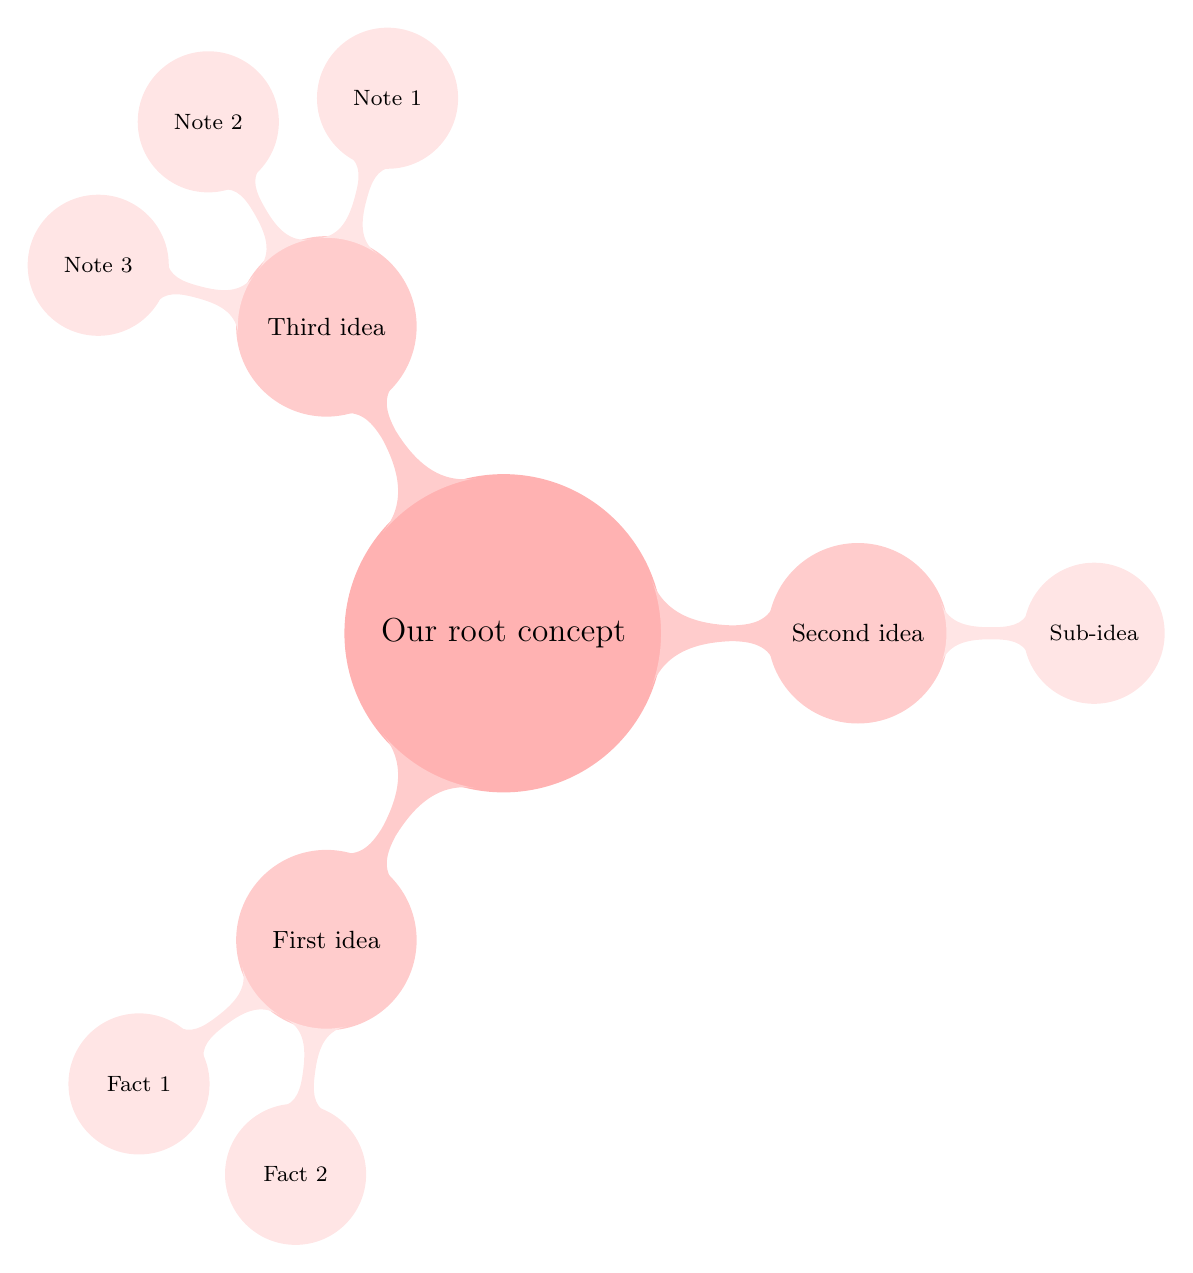
\begin{tikzpicture}[
    mindmap,
    concept color = red!30,
    every node/.style = {concept},
    grow cyclic,
    level 1/.append style = {
        concept color = red!20,
        level distance = 4.5cm,
        sibling angle = 120
    },
    level 2/.append style = {
        concept color = red!10,
        level distance = 3cm,
        sibling angle = 45
    }
]

\node  {Our root concept}
    child {node {First idea}
        child {node {Fact 1}}
        child {node {Fact 2}}
    }
    child {node {Second idea}
        child {node {Sub-idea}}
    }
    child {node {Third idea}
        child {node {Note 1}}
        child {node {Note 2}}
        child {node {Note 3}}
};

\end{tikzpicture}

\end{document}
